% !TEX root = ../../main.tex
\section{\acl{GC} Tools}%
\label{sec:related.constraints}

Constraint-based programming comes in a wide variety of ways, following a
diverse set of programming paradigms, using different approaches to problem
solving briefly detailed in~\cref{sec:intro.constraints}.  Some of them also
support an associative programming model, such as
DesignScript~\cite{Aish:2011:DesignScript}, further discussed in
\cref{sec:related.ad.dynamo}, allowing for the propagation of changes made to a
variable to others that depended on the former.

\Cref{tab:related.constraints.summary} succinctly analyzes tools capable of
solving geometric constraints.  From this table, Eukleides, GeoSolver, and the
\acs{TikZ} \& \acs{PGF} system are further discussed: Eukleides for its elegant
declarative language, similar to some of the languages outlined in
\cref{tab:related.ad.summary}; GeoSolver for its helpful analysis \ac{GUI},
along with the fact it is implemented in Python, a well established and easy to
use language, already used in some competence in \ac{CAD} software (see
\cref{tab:related.ad.summary}); and \acs{TikZ} for its wide support,
development, usage, and collection of packages that extend it, enabling the
specification of graphics and geometry in a variety of simple distinct ways.

\begin{table}[htbp]
  % \small
  \begin{tabularx}{\textwidth}{X*{7}{c}}
    \toprule
    \textbf{Tool}
      & \textbf{\acs{TPL}}
      & \textbf{\acs{VPL}}
      & \textbf{Assoc}$^\dag$
      & \textbf{Decl}$^\ddag$
      & \textbf{Imp}$^\ast$
      & \textbf{2D}
      & \textbf{3D}
    \\\midrule
    DesignScript~\cite{Aish:2011:DesignScript}
      & \checkmark{}
      & \xmark{}
      & \checkmark{}
      & \xmark{}
      & \checkmark{}
      & \checkmark{}
      & \checkmark{}
    \\\midrule
    Eukleides~\cite{Obrecht:2010:EM}
      & \checkmark{}
      & \xmark{}
      & \xmark{}
      & \checkmark{}
      & \checkmark{}
      & \checkmark{}
      & \xmark{}
    \\\midrule
    GeoGebra~\cite{Hohenwarter:2004:CDGACSSG}
      & \checkmark{}
      & \checkmark{}
      & \xmark{}
      & \xmark{}
      & \checkmark{}
      & \checkmark{}
      & \checkmark{}
    \\\midrule
    GeoSolver~\cite{Van:2009:NRCRASSGC,Van:2009:GeoSolver}
      & \checkmark{}
      & \checkmark{}
      & \xmark{}
      & \xmark{}
      & \checkmark{}
      & \checkmark{}
      & \checkmark{}
    \\\midrule
    Kaleidoscope$^\P$~\cite{Lopez:1994:Kaleidoscope}
      & \checkmark{}
      & \xmark{}
      & \checkmark{}
      & \xmark{}
      & \checkmark{}
      & $\approx$
      & $\approx$
    \\\midrule
    ThingLab~\cite{Borning:1989:PLATL}
      & \xmark{}
      & \checkmark{}
      & \checkmark{}
      & \checkmark{}
      & \xmark{}
      & \checkmark{}
      & \checkmark{}
    \\\midrule
    \acs{TikZ} \& \acs{PGF}~\cite{Tantau:2015:tikz-manual}
      & \checkmark{}
      & \xmark{}
      & \xmark{}
      & \xmark{}
      & \checkmark{}
      & \checkmark{}
      & \xmark{}
    \\\bottomrule
  \end{tabularx}
 
  {\scriptsize
  \P{}    --- Doesn't natively support \acs{GCS}, but can be extended to solve
  this class of constraint problems.
  \dag{}  --- Associative model / \textit{change-propagation} mechanism;
  \ddag{} --- Declarative paradigm;
  $\ast$  --- Imperative paradigm
  }

  \caption[Table of tools and languages with \acs{GCS} capabilities]{
    Table of tools and languages with \acs{GCS} capabilities.}%
  \label{tab:related.constraints.summary}
\end{table}

\begin{comment}
\subsection{\acs{CGAL}}%
\label{sec:related.constraints.cgal}

Already partly discussed in \Cref{sec:related.robustness}, \acs{CGAL} is a
compilation of a series of packages, ranging from Arithmetic and Algebra to
Geometric Optimization packages and more.  The main goal of the project is to
provide easy access to efficient and reliable geometric algorithms.

In the form of a C++ library, \acs{CGAL} offers data structures and algorithms
like Voronoi diagrams, geometry processing, complex hull algorithms, among
others.  These operate on geometric objects and perform geometric tests on them.
These objects and predicates are regrouped in \acs{CGAL} Kernels, e.g., the 2D
and 3D Linear Geometry Kernel~\cite{cgal:bfghhkps-lgk23-18b}.  Kernels are
easily interchangeable, allowing the user to pick the underlying number types
and algorithms most appropriate for the given use case, further being capable of
using multiple Kernels simultaneously.
\end{comment}

\subsection{Eukleides}%
\label{sec:related.constraints.eukleides}

A computer language devoted to elementary plane geometry~\cite{Obrecht:2010:EM},
Eukleides is a simple, full featured, and mainly declarative programming
language, capable of handling basic data types, such as numbers and strings, and
most importantly, geometric data types, such as points, vectors, lines, and
circles.  Like most languages, it provides control flow structures, allows user
functions and module definitions, proving for easy extensibility.

Eukleides provides a wide variety of functions and constructions that easily
allow the user to specify geometric constraints between objects, as demonstrated
by \cref{lst:intro.example.parallel.euk,lst:intro.example.circumcenter.euk}.
Among the listed ones, it includes functions to build parallel and perpendicular
lines with respect to another line or segment, determine a line's bisector,
tangent lines to a circle, shape intersection, and so on~\cite{Obrecht:2010:EM}.
Mainly provisioned with two interpreters with the capability of generating
\ac{EPS} files or produce macros, enabling the embedding of Eukleides figures in
\LaTeX{} documents.

Despite heavy support for 2D geometric constructs, as mentioned, it is a tool
that focuses on 2D geometry alone, which arguably leads to its primary
disadvantage: the lack of 3D geometry support.  It is also a \ac{TPL}, which
means that, although being a very simple language, it is less intuitive than a
\ac{VPL}.  The first version of Eukleides included a \ac{GUI},
\texttt{xeukleides}, but one is not yet available for the current version.

Eukleides has not been actively developed for a couple of years, while
\acs{TikZ} still is.  The latter still dominates diagram and graphic production
in \LaTeX{} documents, some people going as far as suggesting opting for it
instead of using the former~\cite{Christian:2014:TEXE:Eukleides}.

\subsection{GeoSolver}% 
\label{sec:related.constraints.geosolver}

GeoSolver is an open-source Python package that provides classes and functions
for specifying, analyzing, and solving geometric constraint
problems~\cite{Van:2009:GeoSolver}.  It features a set of 3D geometric
constraint problems consisting of point variables, two-point distance and
three-point angle constraints.  Problems with other geometric variables can be
mapped to these basic constraints on point variables.

The solution found by GeoSolver is generic and parametric.  It can be used to
derive a specific solution.  Since generic solutions are exponentially hard to
find, GeoSolver also allows two different ways of selecting a solution, reducing
the number of solutions that would be generated, consequently reducing
computation time.  In order to efficiently find a solution, GeoSolver employs a
cluster rewriting-based approach described in~\cite{Van:2009:NRCRASSGC}, capable
of handling non-rigid clusters contrasting with typical graph constructive-based
approaches.

A \ac{GUI} interactive tool called \ac{GCS} Workbench~\cite{DeRegt:2008:WGCS}
(see \cref{fig:related.constraints.geosolver.gcs}) is distributed along with the
GeoSolver package.  The user can easily edit, analyze and solve geometric
constraint problems.  The latter features are obviously supported by GeoSolver,
and 3D interactivity support comes in the form of pyQt and pyOpenGL\@.  An
excellent tool for understanding how a geometric constraint problem is
decomposed in GeoSolver, but not efficient for complex design tasks when
compared with its programmatic supporting package.

\begin{figure}[htbp]
  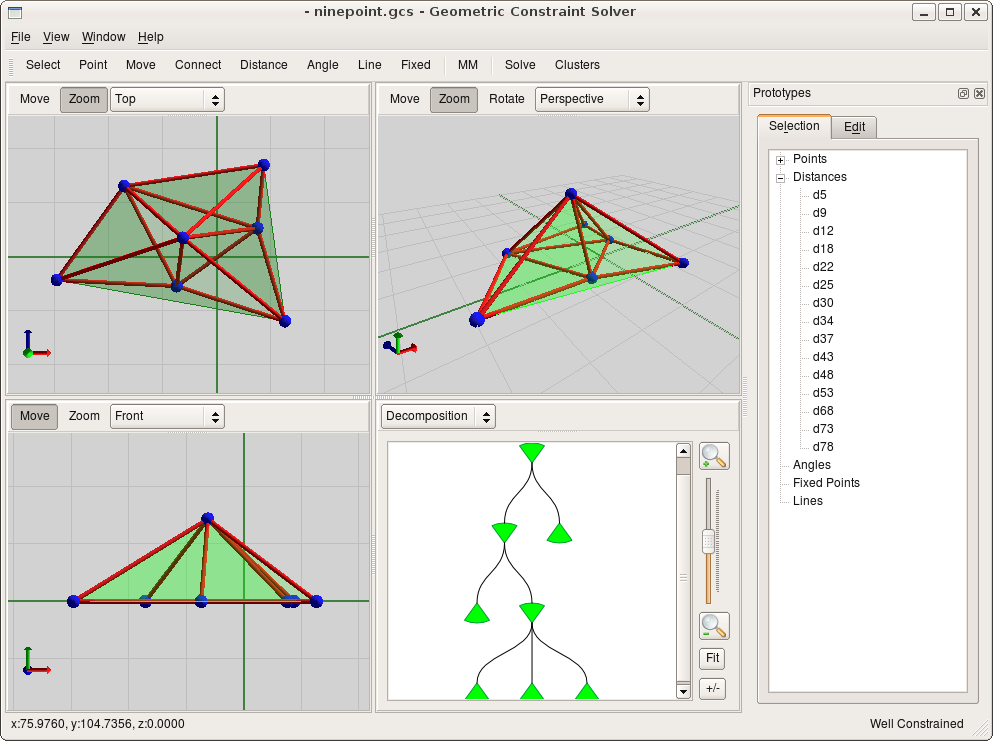
\includegraphics[width=\textwidth]{fig/gcs-workbench}\\
  {\scriptsize
  Source: \url{http://geosolver.sourceforge.net} (Jan 2019)}
  \caption[\acs{GCS} Workbench \acs{GUI}]{
    Depiction of the \acs{GCS} Workbench's visual interface with two
    separate panes:
    \begin{enumerate*}[label= (\arabic*)]
      \item showcasing different perspectives of the model and the constraint
      problem's decomposition, and
      \item a prototyping pane, destined for constraint analysis and edition.
    \end{enumerate*}}%
  \label{fig:related.constraints.geosolver.gcs}
\end{figure}

\subsection{\acs{TikZ} \& \acs{PGF}}%
\label{sec:related.constraints.tikz}

Originally a small \LaTeX{} style created by Till Tantau for his PhD thesis,
\acs{TikZ}~\cite{Tantau:2015:tikz-manual}, along with its underlying lower-level
\ac{PGF} system, is a fully featured graphics language, basically consisting of
a series of \TeX{} commands that draw graphics.  \acs{TikZ} stands for
``\acl{TikZ}\label{acro:TikZ}'', a recursive acronym, which translates to
``\acs{TikZ} is not a drawing program''.  As mentioned, the user instead
programmatically describes their drawings.

On its own, \acs{TikZ} already includes a series of commands capable of handling
geometric constraints, such as tangency, perpendicularity, intersection; but may
appear daunting to the user in its raw form.  Several packages have been built
on top of it to facilitate the generation of drawings using a simpler syntax
such as \texttt{tkz-2d}, a package superseded by
\texttt{tkz-euclide}~\cite{Matthes:2011:tkz-euclide-manual}.  The package
\texttt{tkz-euclide} was designed for easy access to the programming of
Euclidean geometry using a Cartesian coordinate system with TikZ.  It was used
to produce \cref{fig:intro.example} with the respective code listed in
\cref{lst:intro.example.parallel.tikz,lst:intro.example.circumcenter.tikz}.

Like Eukleides, an obvious limitation they share is the lack for 3D modeling
support.  Unlike it, a plethora of resources and usage examples exist, along
with an immense amount of packages that layer on top of it for a panoply of
diverse use cases.  It still undoubtedly remains the go-to graphics system
within the \TeX{} typesetting community.  However, again comparing it to
Eukleides, for example, even using something as \texttt{tkz-euclide}, it can
look syntactically appalling, even for the adept \TeX{} user, instead of
following a simpler and established familiar syntax akin to other declarative or
imperative programming languages.
